\documentclass[11pt,a4paper]{report}
\usepackage{amsmath}
\usepackage{amsfonts}
\usepackage{amssymb}
\usepackage{setspace}
\usepackage{url}
%\usepackage{cite}
\usepackage{fancyhdr}
\usepackage{titlesec}
\titleformat{\subsection}{\itshape\normalsize}{\thesubsection}{1em}{}
% interligne
\usepackage{pdflscape}
\usepackage{placeins}
\usepackage{cite}
\usepackage[left=2cm,
			right=2cm,
			top=3cm,
			bottom=3cm]{geometry}
\author{Cyril Matthey-Doret}
\usepackage{outline} \usepackage{pmgraph} \usepackage[normalem]{ulem}
\usepackage{verbatim}
\pagestyle{fancy}
\setlength{\footskip}{80pt}
% chargement des figures
\usepackage{graphicx}					
\usepackage{wrapfig}
\usepackage[export]{adjustbox}
\usepackage[labelfont=bf]{caption}

\title{

\includegraphics[width=1.75in]{lo_unil06_bleu.pdf} \\
\vspace*{1in}
\textbf{Do enhancer-associated lincRNAs contribute to nuclear architecture ?}}

\author{\Large{First Step Project}\\
		Master in Molecular Life Sciences, Bioinformatics\\
				\vspace*{0.5in} \\
		Cyril Matthey-Doret\\
        Supervised by: Jennifer Yihong Tan\\
        Directed by: Ana Claudia Marques\\
		\vspace*{0.5in} \\
		Department of Computational Biology\\
		Department of Physiology\\
        \textbf{University of Lausanne - Switzerland}\\
       } \date{\today}
%--------------------Make usable space all of page
\setlength{\oddsidemargin}{0in} \setlength{\evensidemargin}{0in}
\setlength{\topmargin}{0in}     \setlength{\headsep}{+0.5in}
\setlength{\textwidth}{6.5in}   \setlength{\textheight}{8.5in}
%--------------------Indention
\setlength{\parindent}{1cm}

\begin{document}

%--------------------Title Page
\renewcommand{\headrulewidth}{1pt}
\fancyhead[R]{First Step Project, University of Lausanne - Switzerland, December 2016}
\maketitle
%--------------------Begin Outline

\section*{Abstract}

A large proportion of the human transcriptome generates RNA products that are not translated into proteins. Intergenic long noncoding RNAs (lincRNAs), are such noncoding RNAs that are longer than 200 nucleotides found within the intergenic spaces of the genome and they represent the largest part of the noncoding transcriptome in humans. Although only less than 1\% of these transcripts have been functionally annotated, they comprise a wide array of regulatory functions. In particular, instances of lincRNAs that originate from enhancer activities (elincRNAs) have been associated with regions of frequent chromosomal contacts, called topologically associating domains (TADs), which ultimately shape the transcriptome landscape of the genome. However, the genome-wide prevalence and impact of elincRNAs on the regulation of chromosomal architecture remain unknown. Here, using data from other functional genomics studies in human lymphoblastoid cells, I investigated the global role of elincRNAs in the spatial organization of the genome. Specifically, I found elincRNAs to co-localize with chromosomal loop anchors and binding sites of proteins known to promote chromosomal contacts, suggesting their likely biological relevance in modulating nuclear conformation.

\section*{Introduction}
It was only discovered in the past decade that a surprisingly large proportion of the mammalian transcriptome does not code for proteins. To date, the number of annotated noncoding genes longer than 200 nucleotides (long noncoding RNA, lncRNA) exceeds that of protein-coding genes by at least 3 times \cite{Iyer2015}⁠. Amongst all lncRNAs, those that do not overlap protein-coding genes, referred to as long intergenic noncoding RNAs (lincRNAs), are the most abundant. Functional and evolutionary analyses, together with extensive characterization of a handful of lincRNAs, have demonstrated that some of these transcripts are involved in the regulation of gene expression programs, both transcriptionally and post-transcriptionally, and that they can contribute to organismal traits and diseases \cite{Kornienko2013}⁠. However, the mechanisms and functions, if any, for the majority of lincRNAs remain unknown \cite{Rinn2012}⁠.  

A large proportion of lincRNAs originate from active enhancers. These enhancers are widely transcribed and generate noncoding products, broadly classified as enhancer-associated noncoding RNAs (eRNAs). eRNAs can be bidirectional non-poly-adenylated or unidirectional poly-adenylated. The latter include lincRNAs, which are referred to as enhancer-associated lincRNAs (elincRNAs) \cite{Guil2012}. 

Recently, a set of such enhancer-derived lincRNAs that were associated with human trait variants, were shown to regulate local gene expression in \textit{cis} in human lymphoblastoid cell lines (LCLs). Importantly, higher frequencies of chromosomal interactions are often observed at these loci relative to other lincRNAs, suggesting that elincRNAs may be involved in gene regulation through modulating chromatin architecture (Tan et al, 2016, under revision).

Gene regulation is shaped by spatial organization of the genome \cite{Engreitz2016}⁠⁠. Specifically, the folding of genomic DNA into variably compact chromosomal structures can strongly influence expression of the embedded genes \cite{Gorkin2014}⁠⁠. Globally, regions with low degree of compaction, referred to as euchromatin, are associated with high levels of active transcription. On the other hand, relatively condensed and less transcriptionally active regions are called heterochromatin \cite{Passarge1979}\cite{Tamaru2010}⁠. Chromosomes are further compartmentalized into smaller domains, called topologically associating domains (TADs), where frequent DNA:DNA interactions occur as a result of their close spatial proximity. These domains are key in modulating gene transcriptional programs. Recent findings show that regions near TAD borders, called TAD boundaries, are essential for modulating gene regulatory interactions within TADs and preventing chromatin contacts between TADs. Deletion of TAD boundaries can disrupt those interactions, resulting in gene misexpression and disease phenotypes \cite{Lupianez2015}⁠.

Detailed functional characterizations of a few elincRNAs have established the molecular mechanisms underlying their roles in the spatial organization of the genome. For example, Haunt is one such elincRNA \cite{Yin2015}⁠⁠, which regulates the expression of the HOXA gene cluster by modulating intrachromosomal looping. These recent findings raise the question on what is the prevalence of elincRNAs contributing to gene regulation through modulating chromosomal conformation.

Using publicly available multi-omics data from human LCLs. I investigated the functional role and prevalence of elincRNAs in nuclear organization. Specifically, I examined their enrichment in regions that are key in TAD regulation and their association with the amount of chromosomal interactions to gain initial insights into their roles in gene regulation within topological domains. My analyses show that elincRNAs are associated with high density of DNA:DNA contacts within TADs and are significantly enriched in binding sites of proteins important for TAD regulation. Importantly, elincRNAs are strongly enriched at chromosomal loop anchors where promoter-enhancer interactions are frequent. Together, my findings support the hypothesis that elincRNAs may contribute to gene regulation by establishing contacts between gene regulatory elements and modulating chromosomal organization.

\section*{Results}

Enhancer-associated lincRNAs (elincRNAs) in human lymphoblastoid cell lines (LCLs) were identified from a set of LCL-expressed lincRNAs (Tan et al, 2016, under revision). They were defined based on overlap between their putative promoter regions (estimated as 1kb upstream from their transcriptional start site) and enhancers predicted from histone marks in LCL (GM12878, \cite{ENCODEProject2012}⁠). LincRNAs whose promoter region also overlapped other predicted regulatory elements, specifically active promoters \cite{ENCODEProject2012}⁠, in LCLs were excluded from the analysis (elincRNAs=236, other LCL-expressed lincRNAs=1756).

\subsection*{elincRNAs show similar expression profiles as other lincRNAs}

Most enhancer-associated noncoding RNAs (eRNAs) are transcribed bidirectionally and then rapidly degraded by the nuclear exosome, which makes them hard to detect due to their low expression levels \cite{Darrow2013} \cite{Lam2014}⁠. In contrast, elincRNAs are more stably and preferentially transcribed in a single direction, and are often spliced and polyadenylated \cite{Marques2013a}⁠. 
First, to investigate if LCL-expressed elincRNAs share similar expression profiles relative to other expressed genes as the lowly expressed eRNAs, I compared  their expression levels to that of other lincRNAs and protein-coding genes (Figure \ref{charac_elinc}A). I found that elincRNAs are not expressed at lower levels than other LCL-expressed lincRNAs (GM12878, two-tailed Mann-Whitney U test, $p=0.258$). In addition, contrary to the highly tissue specific eRNAs \cite{Wu2014}, elincRNAs are no differently tissue-specific from other LCL-expressed lincRNAs either, although their median tissue specificity index (Tau) is slightly higher (two-tailed Mann-Whitney U test, $p=0.38$, Figure \ref{charac_elinc}B). These results suggest that elincRNAs may have distinct properties compared to other enhancer-associated transcripts.

\subsection*{elincRNA transcripts are less conserved than other lincRNAs}

To gain insights into the molecular evolution of elincRNAs, I investigated the nucleotide conservation of their exons in primates and placental mammals using phastCons scores \cite{Siepel2005}⁠, a measure of nucleotide conservation (Methods). I found that exons of elincRNAs are less conserved than other LCL-expressed lincRNAs (two-tailed Mann-Whitney U test, mammals: $p<1e-07$, primates: $p<1e-05$) as well as  protein coding genes (two-tailed Mann-Whitney U test, mammals: $p<1e-97$, primates: $p<1e-86$) (Figure \ref{charac_elinc}C). 

Interestingly, a recent study of a set of trait-relevant and enhancer-associated lincRNAs showed that although exons of these lincRNAs did not seem to have evolved under purifying selection relative to other LCL-expressed lincRNAs across mammalian and primate evolution, their sequences are constraint specifically during recent human evolution (Tan et al, 2016, under revision). Therefore, although my result may suggest that elincRNA transcripts were not evolving under constraint across broad mammalian evolution, their conservation across modern human evolution remains to be investigated.

\subsection*{elincRNA promoter regions co-localize with loop anchors and cohesin binding sites}

Next, to examine whether elincRNAs are associated with the regulation of chromosomal architecture, I investigated their co-localization with loop anchors, where enhancer-promoter gene regulatory interactions are frequent \cite{Ji2016}. These regulatory regions are essential to establish chromosomal interactions within topologically associating domains (TADs). I compared the overlap of elincRNAs with these regions relative to what would be expected if these loci were randomly distributed across the intergenic regions of the genome (Methods). I found that elincRNAs are significantly enriched at LCL loop anchors (fold enrichment = 2.79, $q=1e-04$, Figure \ref{enrich_elinc}A).


Architectural proteins, such as cohesin and CTCF, are also enriched at the loop anchors \cite{Rao2014}⁠. Specifically, the cohesin protein-complex is important for cell type-specific intra-TAD gene regulation \cite{Hadjur2009}⁠. The transcription factor CTCF is another central player in the regulation of chromatin architecture and gene expression. According to a recent model \cite{Ji2016}⁠, loops mediated by CTCF only or CTCF and cohesin collectively are important for the structural maintenance of TADs. These loops act as insulators, preventing interactions between TADs. In contrast, loops anchors bound only by cohesin are crucial in mediating regulatory intra-chromosomal interactions, supported by the evidence that cohesin depletion is associated with disrupted promoter-enhancer interactions within TADs \cite{Seitan2013}⁠.

I found that elincRNA promoter regions are significantly enriched in both CTCF and cohesin binding sites in LCL (fold enrichment = 5.2 and 8.1, respectively, $q=1e-04$, union of binding sites for cohesin subunits SMC3 and RAD21 are used to identify cohesin binding, Methods). This enrichment is greater than the one found for other LCL-expressed lincRNAs (fold enrichment = 1.3 and 1.3, $q<0.05$, Figure \ref{enrich_elinc}B) for both CTCF and cohesin binding sites.

Because loops mediated by CTCF and cohesin synergistically are thought to have different roles in chromosomal organization from those mediated by cohesin only  \cite{Ji2016} and a large proportion of binding sites for CTCF and cohesin overlap in the human genome (Figure \ref{enrich_elinc}C)⁠, I further determined the independent enrichment of elincRNAs in CTCF- and cohesin-only binding sites, using mutually exclusive binding sites for these proteins. This revealed a greater enrichment of cohesin binding sites (Figure \ref{enrich_elinc}D) in elincRNA loci (fold enrichment = 13.1, $q=1e-04$) compared to that of CTCF (fold enrichment = 3.92, $q=1e-04$). This suggests elincRNAs are more frequently involved in the formation of cohesin-only loops, supporting their roles in modulating promoter-enhancer looping.

\subsection*{elincRNA promoter regions are not enriched at TAD boundaries}

As loop anchors are frequently found at TAD boundaries, I next investigated whether similar enrichment would be observed for elincRNAs at TAD boundaries. Using Hi-C data (Figure \ref{TAD_loop_def}) I defined TAD boundaries as regions extending inside TADs from the borders until reaching local intra-TAD contacts that exceeds a cut-off threshold (see Methods for details). Although elincRNAs promoter regions are enriched at loop anchors relative to other LCL-expressed lincRNAs, no significant enrichment was found for these loci  at TAD boundaries (fold enrichment = 1.2, $q=0.08$, Figure \ref{enrich_boundaries}A). Despite the absence of significant elincRNA enrichment at TAD boundaries, dividing TADs into 10 equally sized bins reveals that elincRNAs tend to be more frequently found near the end of the TADs and are depleted in the center of the TADs (bin 5, fold enrichment = 0.37, $q=0.06$) relative to other LCL-expressed lincRNAs (Figure \ref{enrich_boundaries}B). The trend is consistent with their enrichment at loop anchors, which also are enriched at TAD boundaries (fold enrichment =1.74 , $q<1e-3$).

This lack of significant enrichment of elincRNAs at TAD boundaries may be a consequence of poor resolution of the current Hi-C technology, which is restrained to a maximum of 5kb \cite{Rao2014}⁠, as well as limitations in the method I have applied to define boundary regions. Briefly, I defined TAD boundaries by extending inwards from TAD borders (see Methods for details), therefore all genes located outside of defined TADs but lying close to a TAD border would be unaccounted for in the analysis. 


\subsection*{elincRNA are associated with high DNA:DNA contacts within TADs}

To further support their role in regulating promoter-enhancer contacts, I investigated whether elincRNAs are associated with regions with higher DNA:DNA interactions. To this end, I measured the average amount of contact within their respective TADs (Figure \ref{TAD_TAD_contacts}A, Methods). I found that elincRNAs are frequently embedded within TADs with a higher average density of contacts compared to other lincRNAs in GM12878 (Fold difference of median contacts=1.24, two-tailed Mann-Whitney U test, $p<1e-04$, Figure \ref{TAD_TAD_contacts}B). In addition, the fold difference in the amount of DNA contacts within TADs that harbour these elincRNA loci relative to other LCL-expressed lincRNAs were less pronounced in the 3 other cell lines investigated (Fold difference in median contacts=1.05, 1.07, and 1.04, p=$0.02, 0.04, 0.472$ in HUVEC, K562 and NHEK, respectively). This suggests that the association between elincRNA expression and chromosomal contacts is likely cell line-dependent. 
Although my findings do not provide insights into the molecular mechanisms through which elincRNAs may regulate chromosomal architecture, their associated high DNA:DNA contacts, together with their enrichment for cohesin binding suggest a role for elincRNAs in the modulation of enhancer-promoter looping within topologically associating domains.

\section*{Figures, tables and legends}

\begin{figure}[ht]
	%\centering
	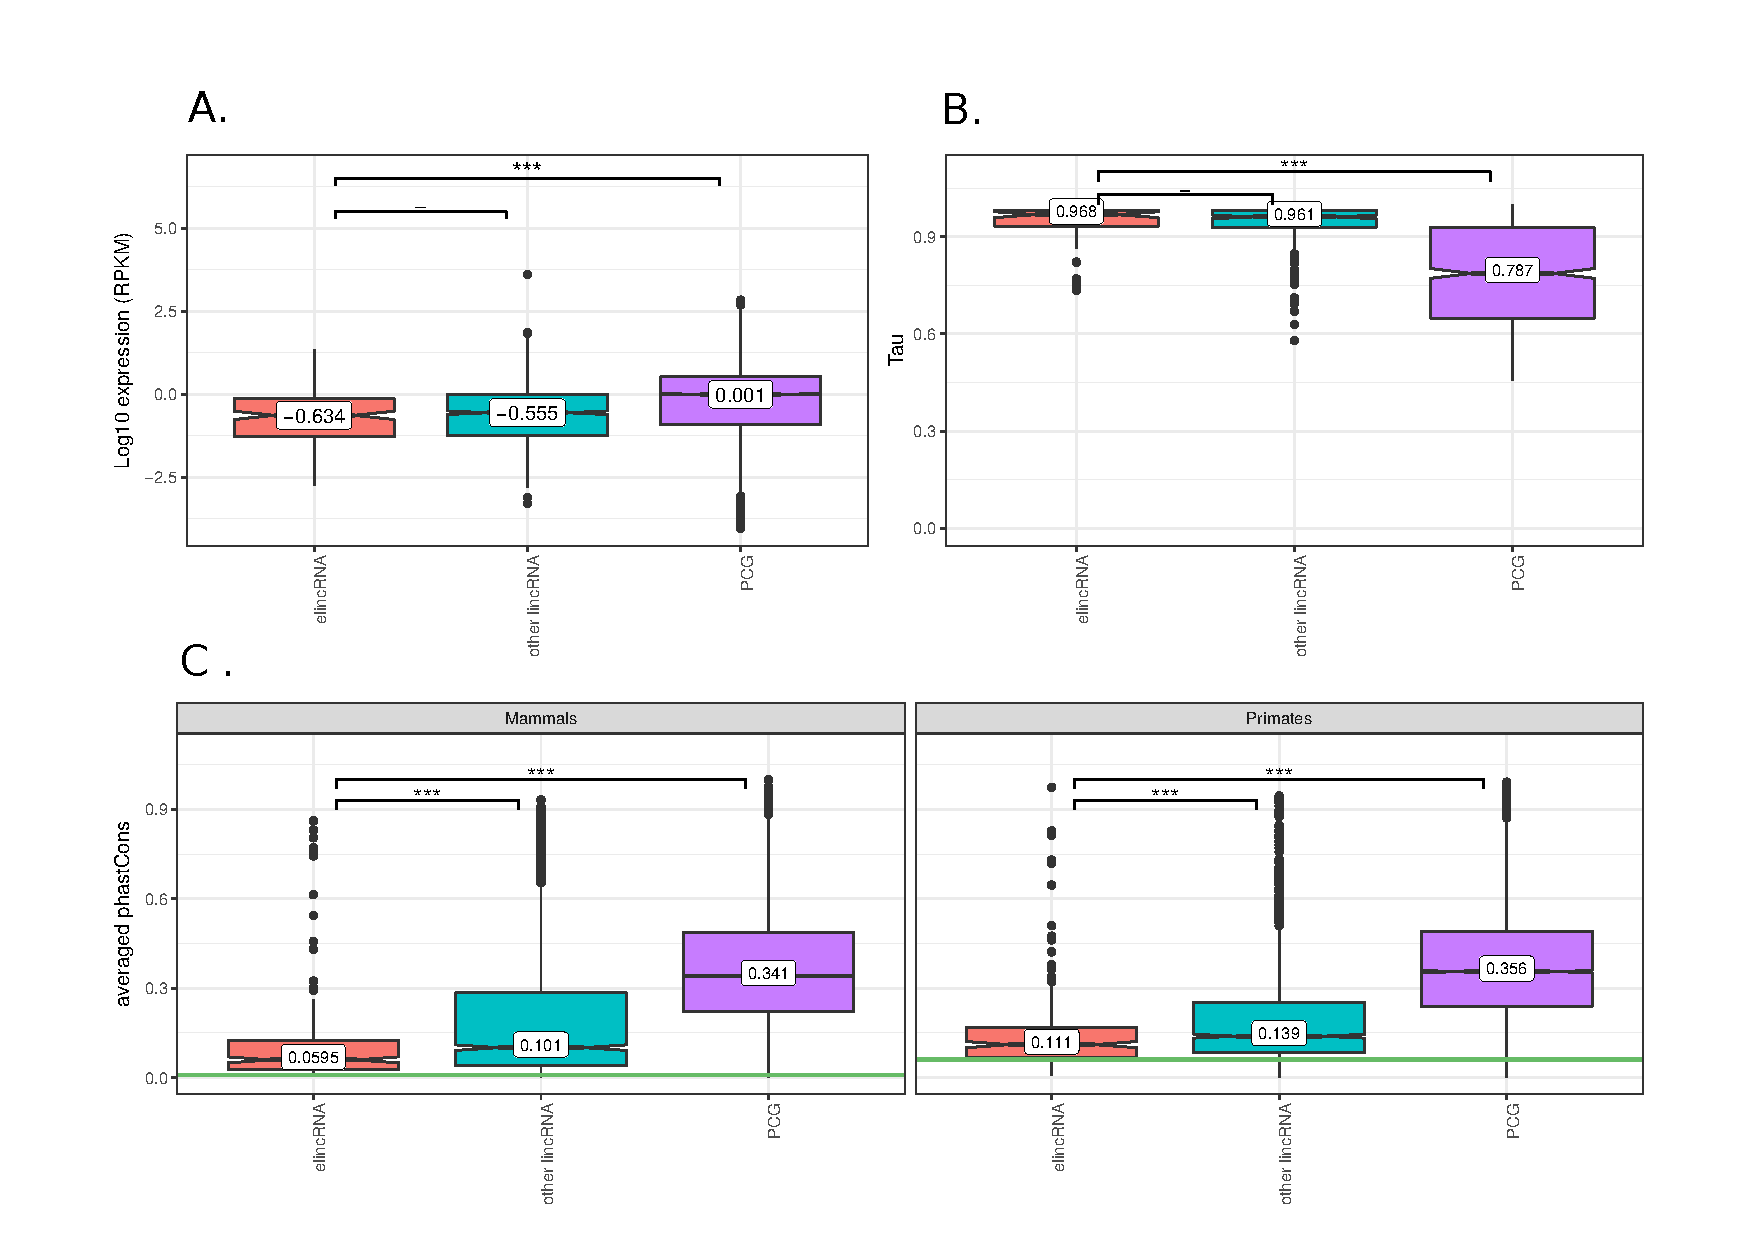
\includegraphics[width=1\textwidth]{Figures/1_full_characterization_elincRNA.pdf}
	\caption{Properties of elincRNAs. \textbf{A.} Distribution of median expression levels in LCL (GM12878), \textbf{B.} tissue specificity index (Tau) and \textbf{C.} Average exonic sequence conservation across mammalian and primate evolution of elincRNAs (orange), other LCL-expressed lincRNAs (blue) and protein-coding genes (purple). The tau index, a measure of gene expression tissue specificity, ranges from 0 (low specificity) to 1 (high specificity)\cite{Kryuchkova2015a}. Average phastCons score is used as a measure for nucleotide conservation \cite{Siepel2005}. The green horizontal line represents the median conservation of ancestral repeats, which are used as a proxy for neutral evolution. Median values of distributions are displayed in the boxes. Differences between distributions were tested using a two tailed Mann-Whitney U test, $***P<0.001$; - not significant}
	\label{charac_elinc}
\end{figure}

\begin{figure}[ht]
	%\centering
	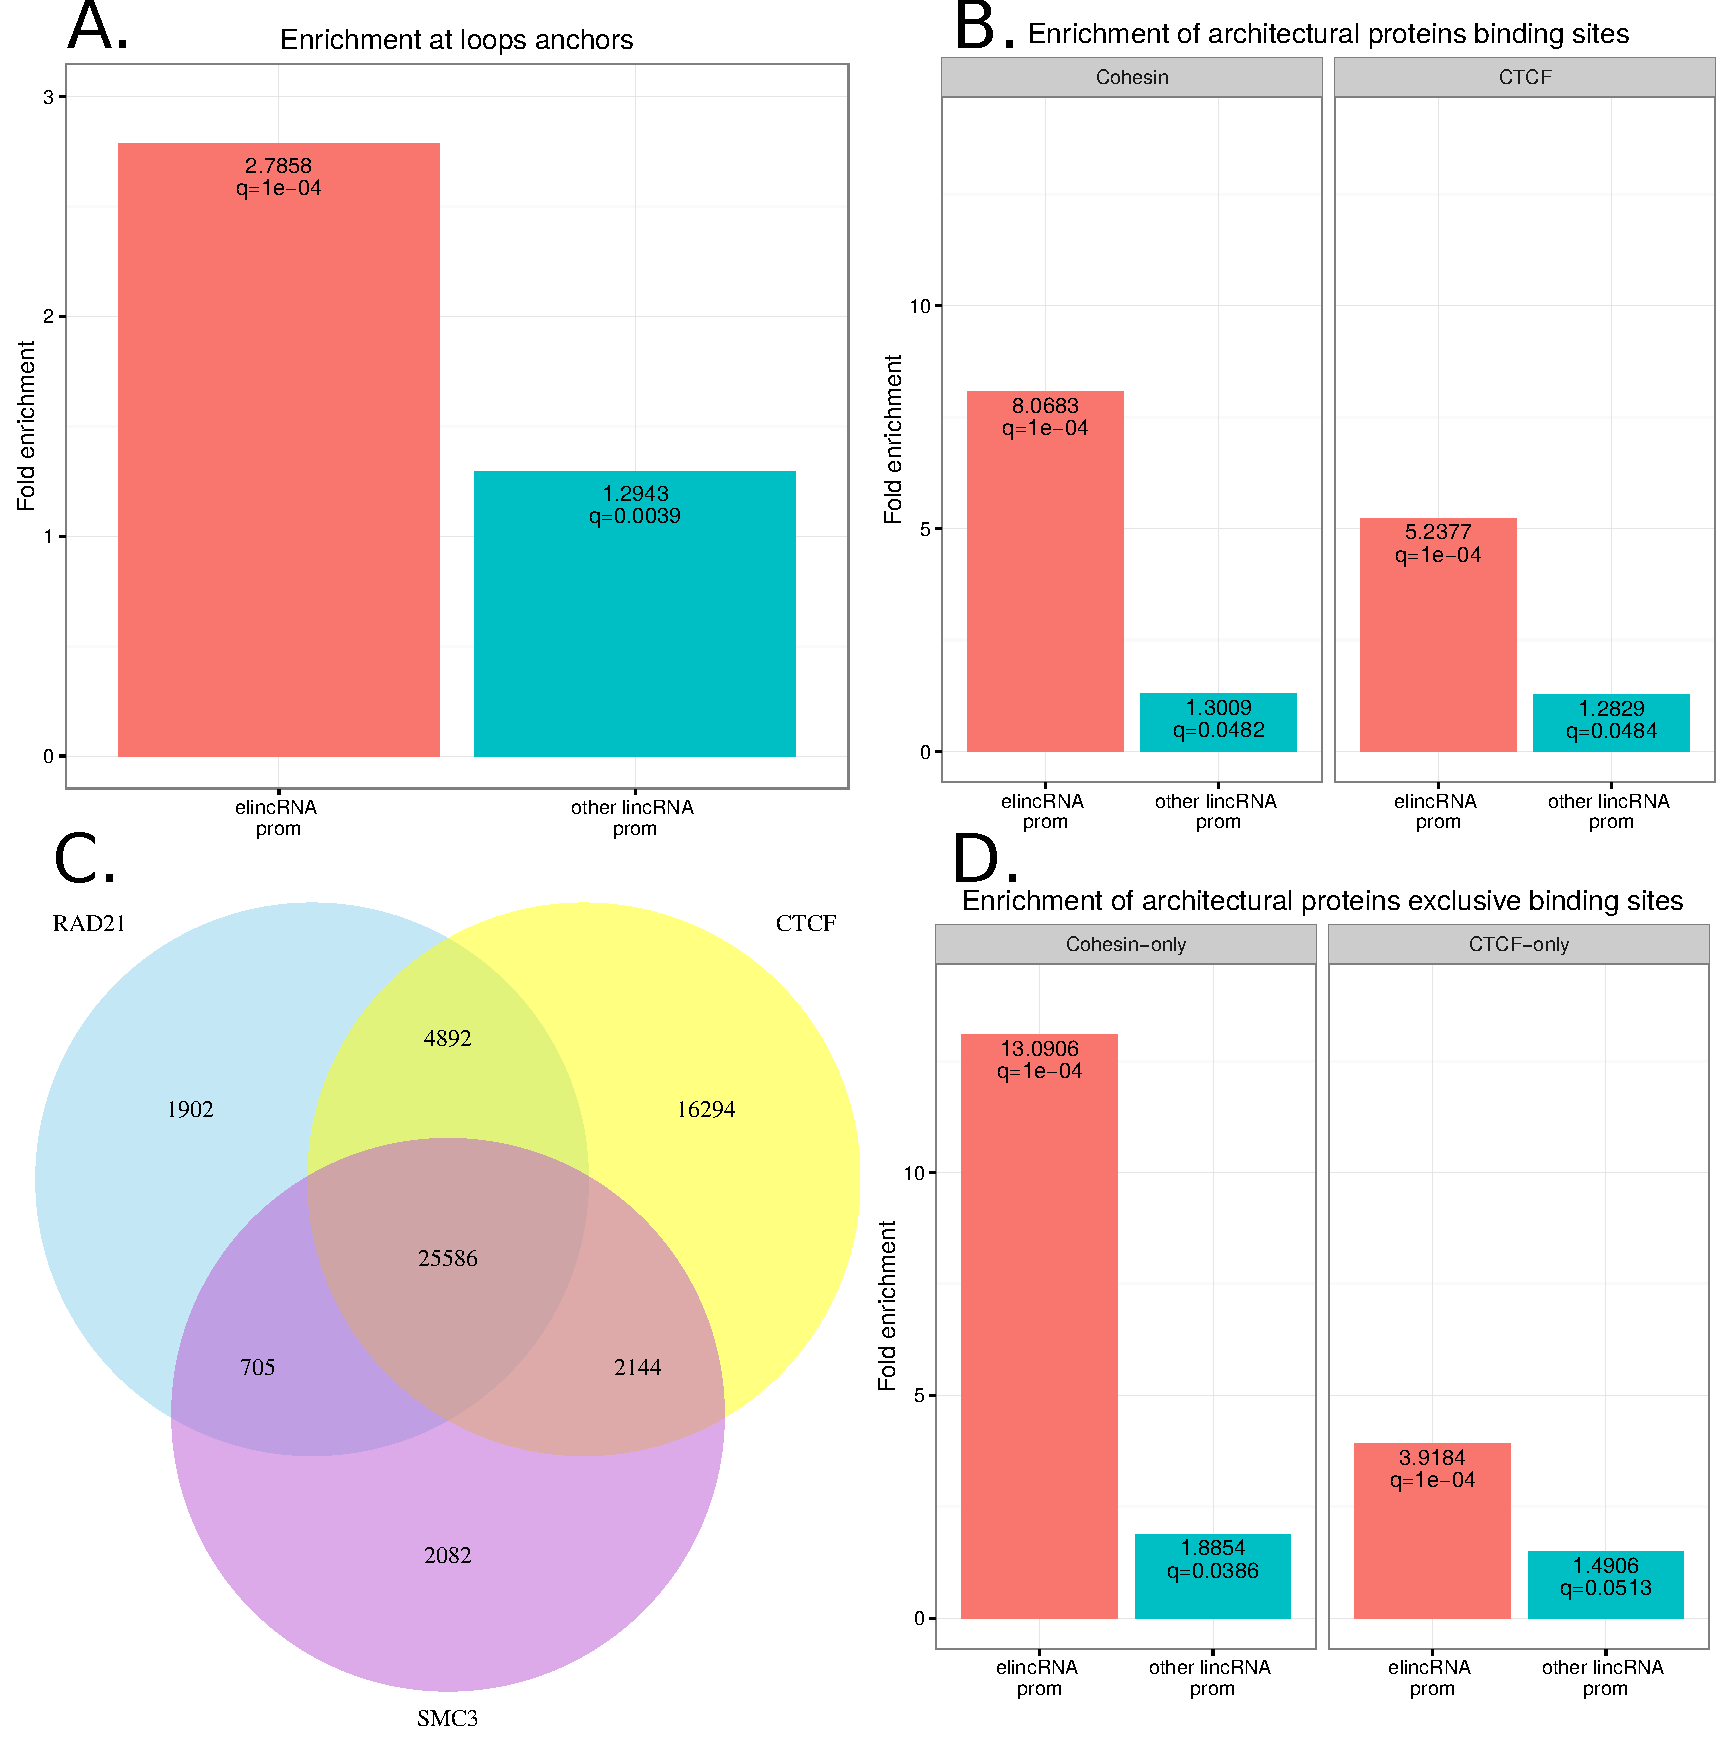
\includegraphics[width=0.9\textwidth]{Figures/2_enrich_anchor_prot.pdf}
	\caption{elincRNAs co-localize with loop anchors and cohesin binding sites. Fold enrichment relative to random expectation: \textbf{A.} elincRNA (red) and other LCL-expressed lincRNA (blue) promoter regions at loop anchors. \textbf{B.} all cohesin and CTCF peaks in human LCLs at elincRNA and other LCL-expressed lincRNA promoter regions. \textbf{C.} Proportions of overlap between cohesin (RAD21 and SMC3) and CTCF peaks in human LCLs. \textbf{D.} cohesin- and CTCF-only peaks at elincRNA and other LCL-expressed lincRNAs promoter regions.}
	\label{enrich_elinc}
\end{figure}

\begin{figure}[ht]
	%\centering
	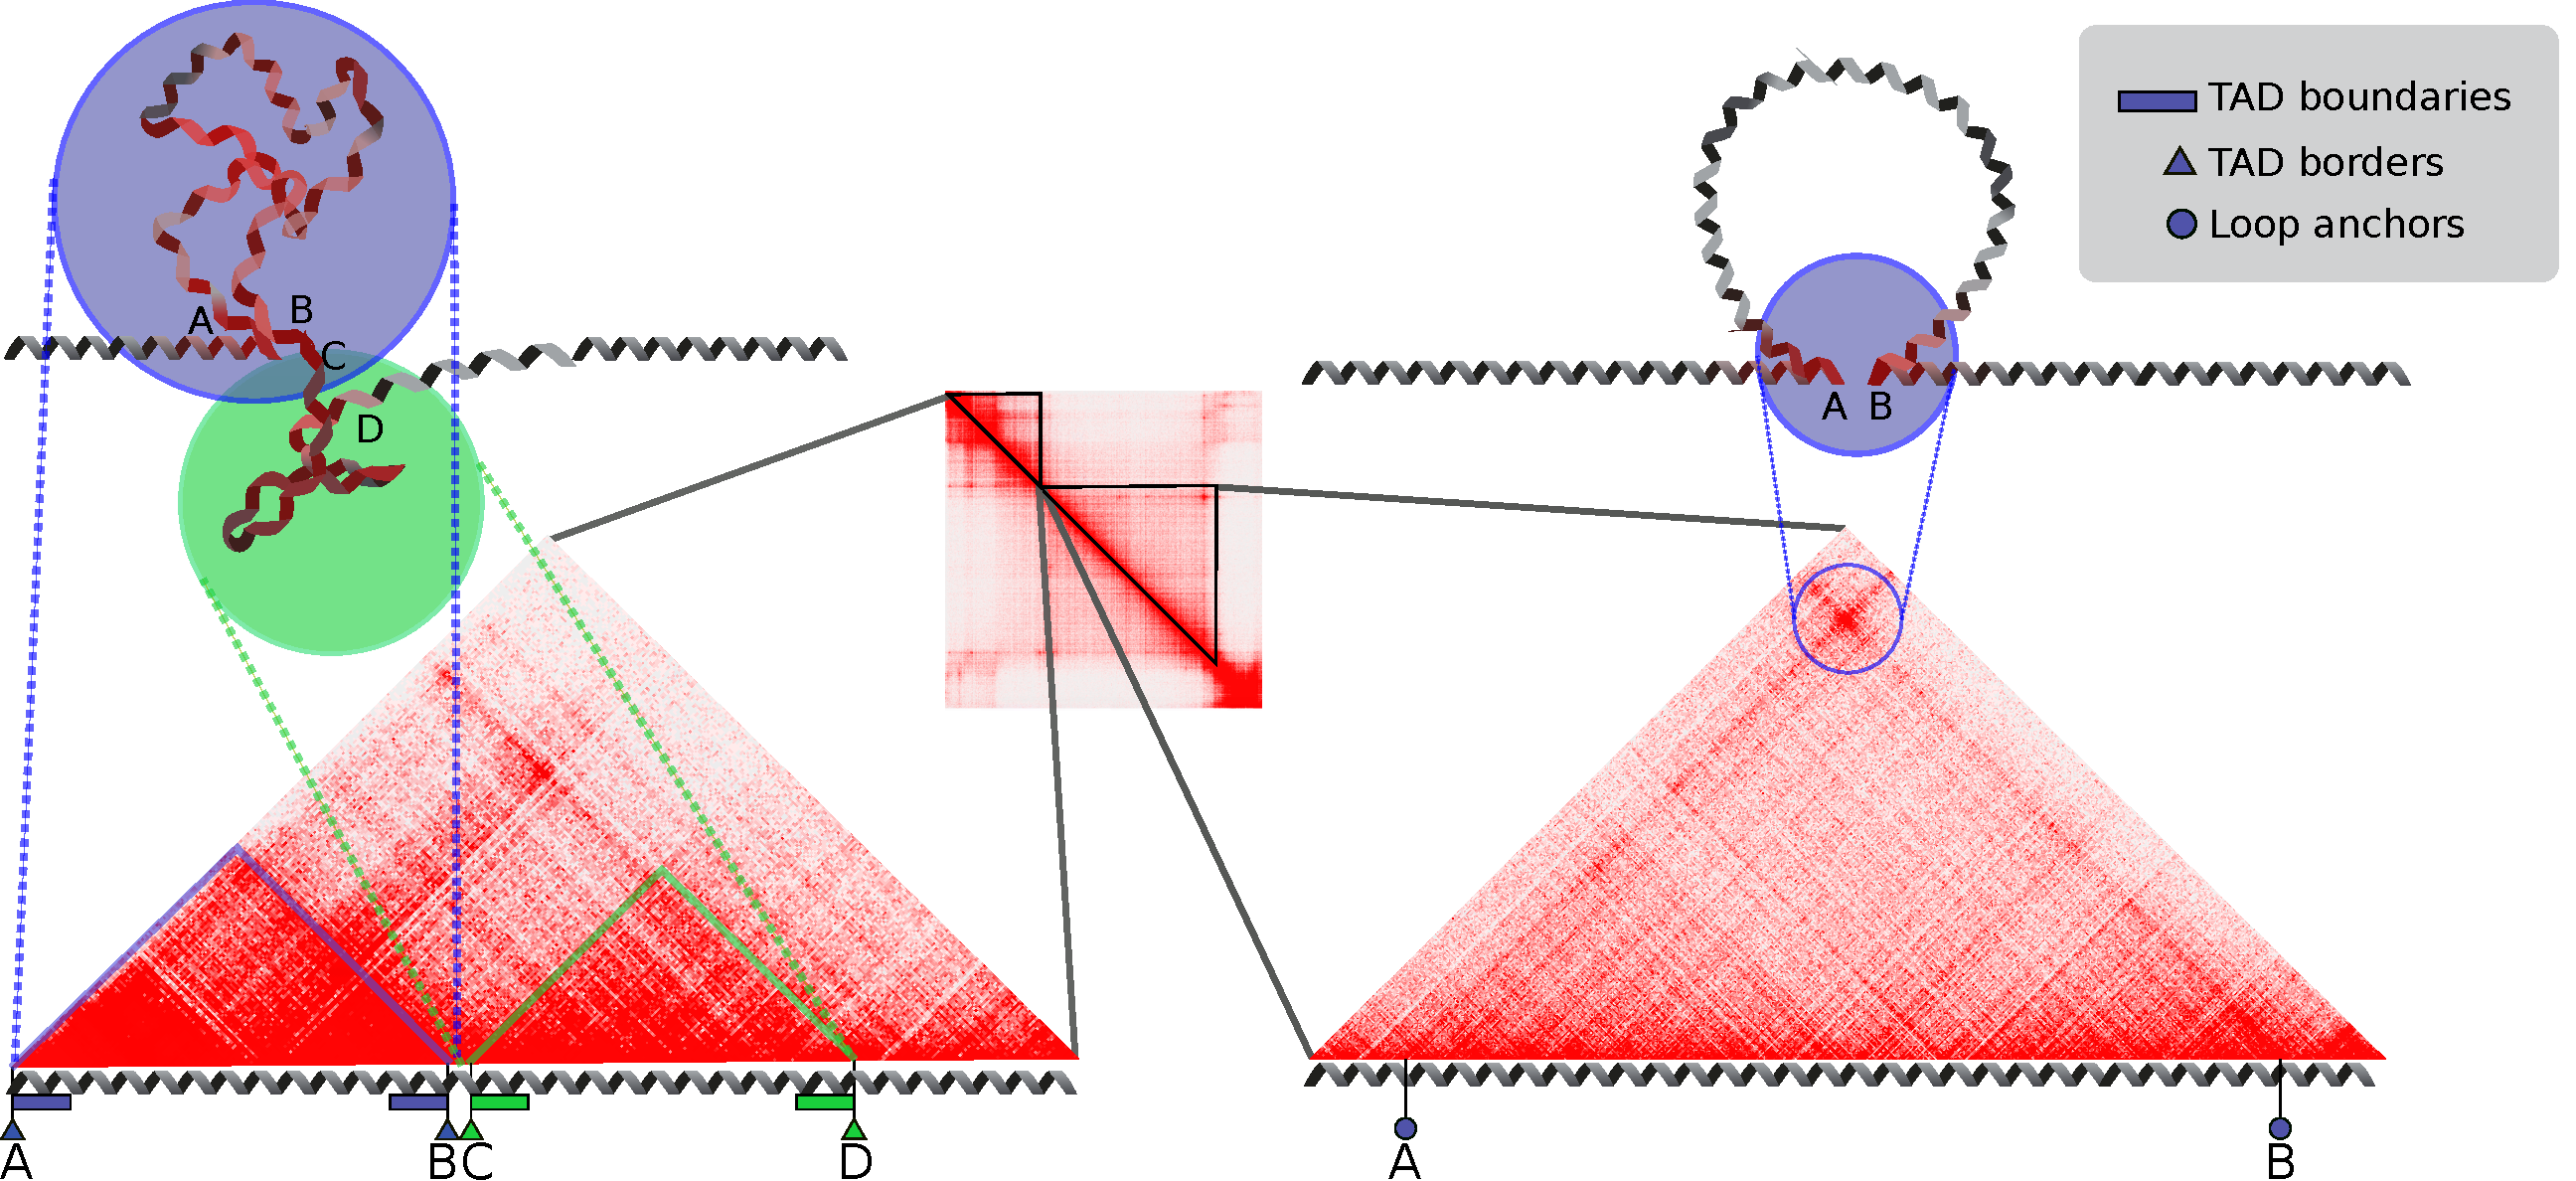
\includegraphics[width=1\textwidth]{Figures/3_TAD_loop_definition.pdf}
	\caption{Schematic representation of topologically associating domains (TADs) and loops using Hi-C matrices. \textbf{A.} TADs and \textbf{B.} chromatin loop represented on a Hi-C intra-chromosomal contact matrix visualized as a symmetrical square matrix (center panel) using Juicebox (Durand et al., 2016)⁠ and as upper triangles, for simplified representation (side panels). Colour intensity of matrix pixels reflect the density of interactions. Left panel: Two TADs are illustrated as two triangular sub-matrices (triangles with blue and green outlines). Frequent interactions occur within these regions while interactions across TADs are less frequent. These two TADs correspond to the two globular chromatin structures within the blue and green circles. a and b denote the borders of the first TAD while c and d represent the borders of the second TAD. Boundaries (blue and green rectangles) are expanded inwards from the borders. Right: Chromosomal loop with a and b representing the loop anchors. Unlike TADs, strong DNA:DNA contact is observed only at the contacting point between loop anchors, while less frequent contact occurs in the region between the two anchor points. }
	\label{TAD_loop_def}
\end{figure}

\begin{figure}[ht]
	%\centering
	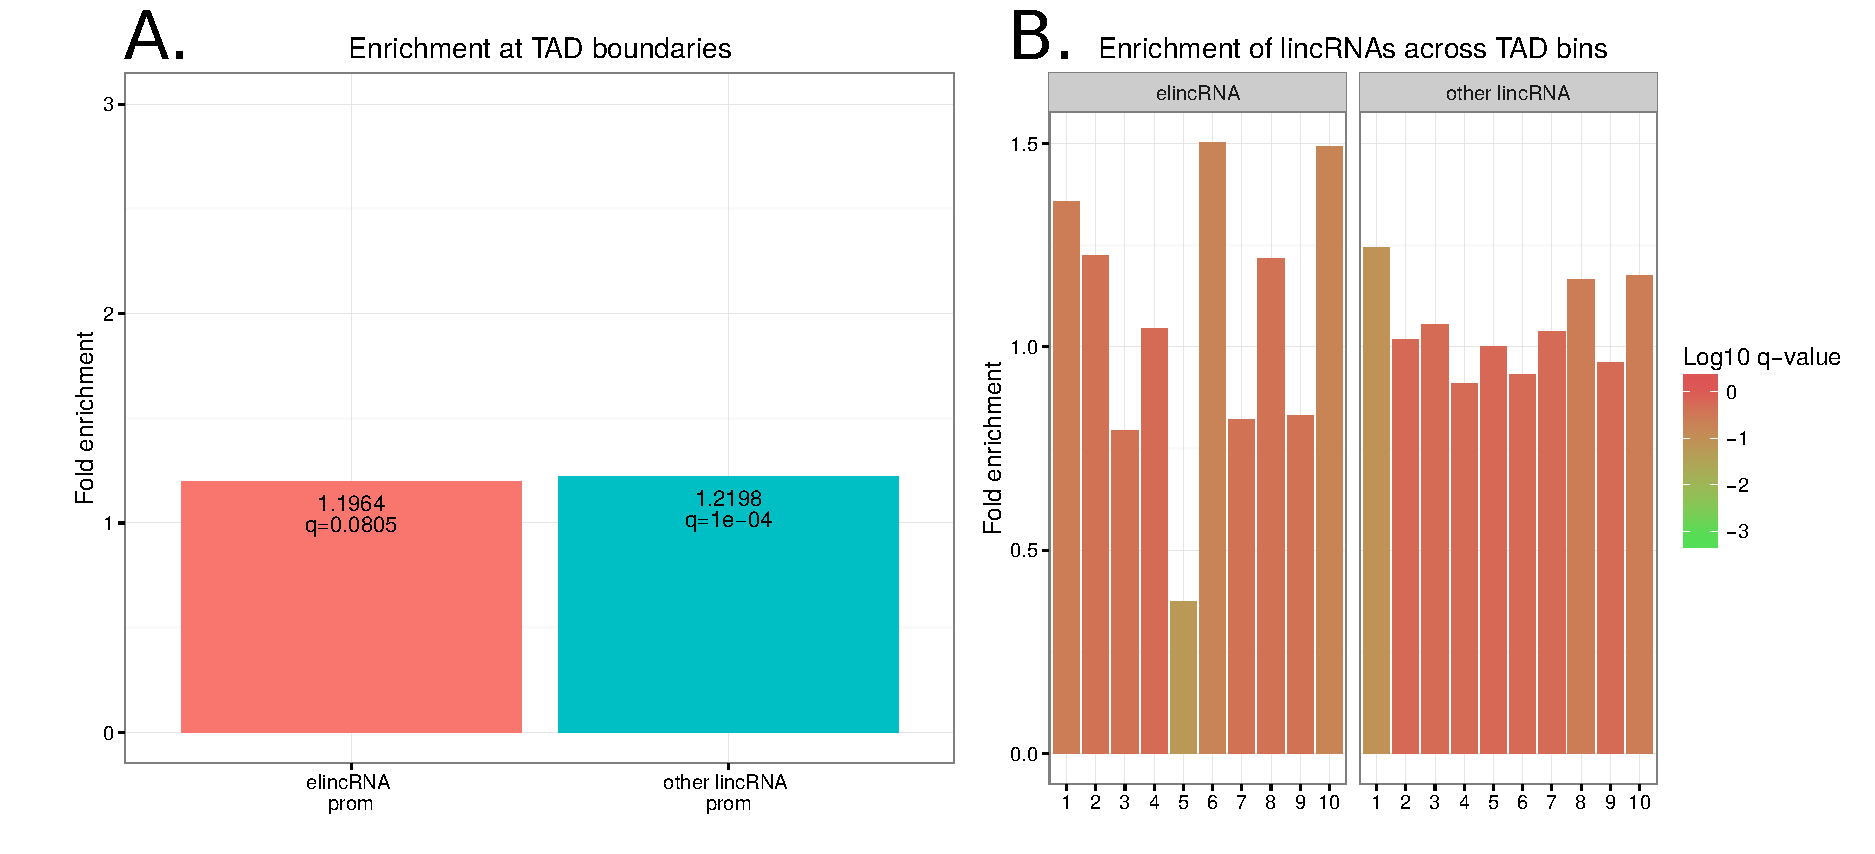
\includegraphics[width=1\textwidth]{Figures/4_enrich_boundaries.pdf}
	\caption{elincRNAs are not enriched at TAD boundaries. Enrichment of elincRNA (orange) and other LCL-expressed lincRNAs (blue) promoter regions \textbf{A.} at TAD boundaries and \textbf{B.} across TADs. Each bar represent a bin containing 10\% of TAD length. Colour of enrichment bars represent log10 of q-values. }
	\label{enrich_boundaries}
\end{figure}

\begin{figure}[ht]
	%\centering
	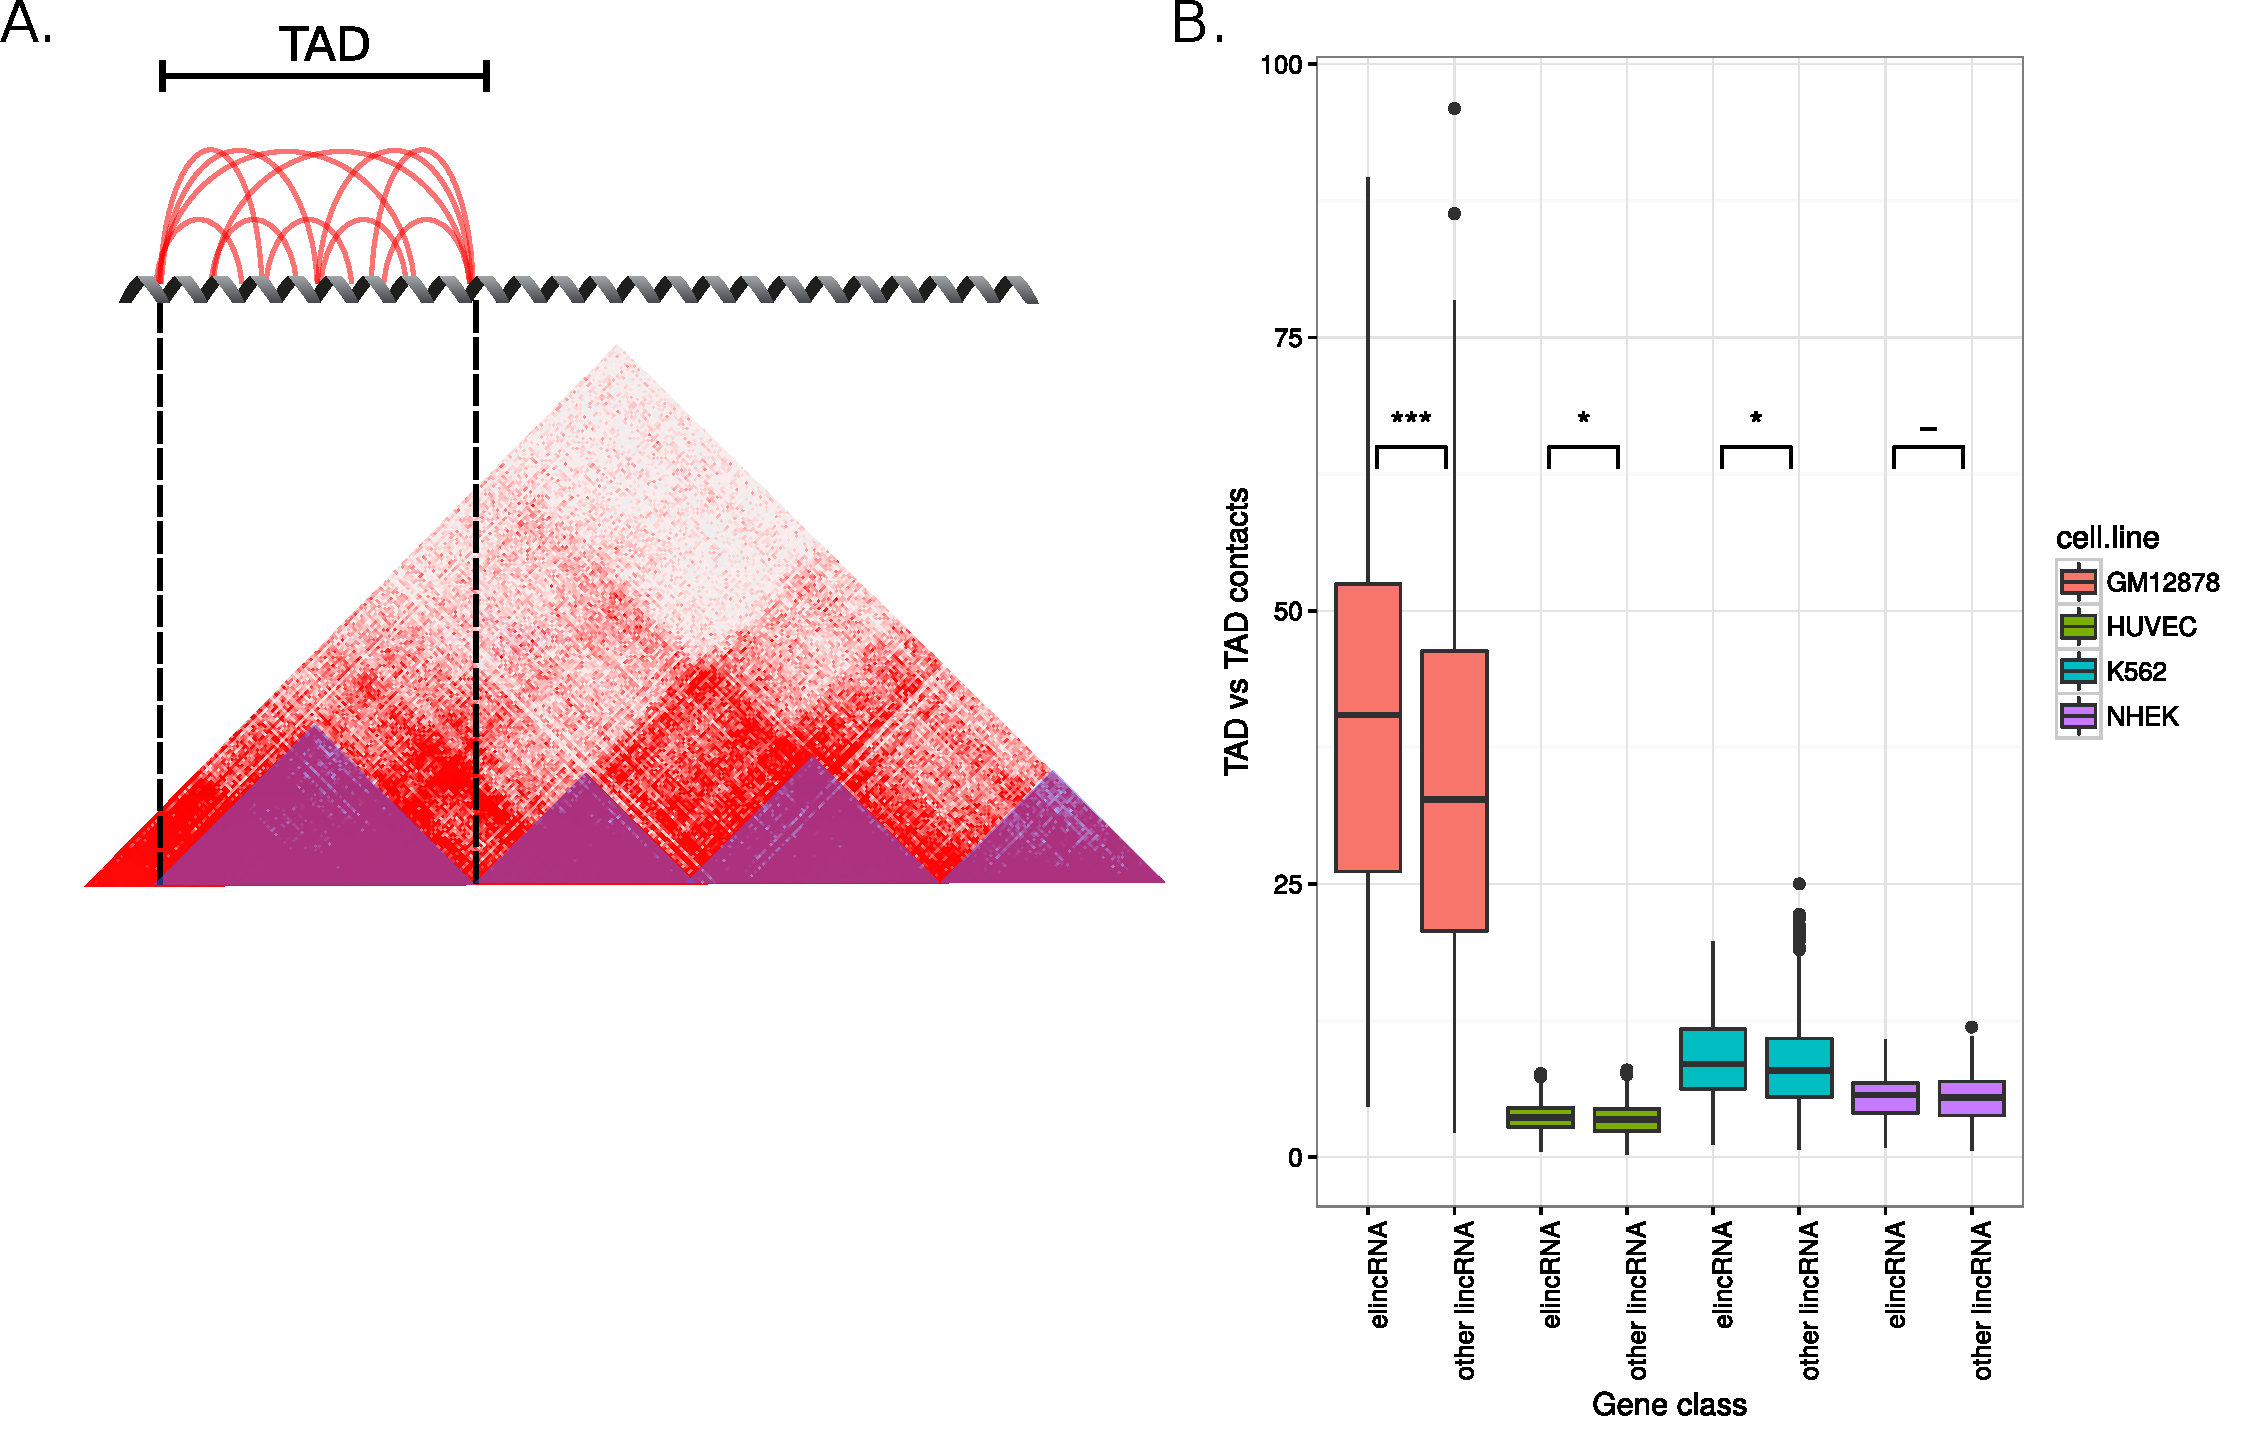
\includegraphics[width=1\textwidth]{Figures/5_TAD_TAD_contact.pdf}
	\caption{elincRNA-containing TADs are associated with significantly higher density of DNA:DNA contacts. \textbf{A.} Mean of interactions within each TAD is computed by summing all DNA contacts within the TAD (purple triangles) and dividing by TAD length. \textbf{B.} Average contact frequency within TADs that encompass elincRNA and other LCL-expressed lincRNAs across four cell lines, GM12878 (orange), HUVEC (green), K562 (blue) and NHEK (purple). Set of genes as defined in GM12878 are used for all comparisons. Difference between groups are tested using the two tailed Mann-Whitney U test, $***P<0.001; *P<0.05$; $-$ non-significant}
	\label{TAD_TAD_contacts}
\end{figure}

\begin{figure}[ht]
	%\centering
	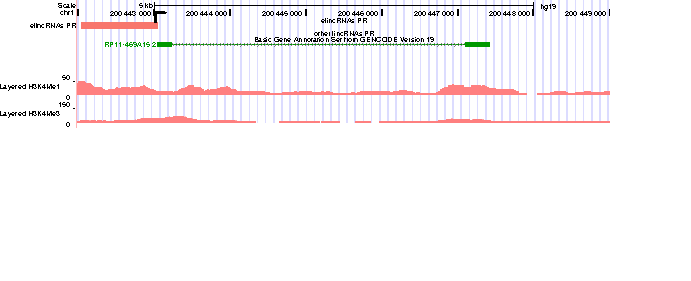
\includegraphics[width=1\textwidth]{Figures/7_merged_examples.pdf}
	\caption{Genome browser view of an elincRNA. \textbf{A.} elincRNA (green) with putative promoter region in pink. The promoter region has low levels of promoter (H3K4Me3) and high level of enhancer (H3K4Me1) histone marks. Exons are depicted as solid boxes and introns as thin lines. The black arrow indicate direction of transcription}
	\label{Genome_browser}
\end{figure}

\begin{figure}[ht]
	%\centering
	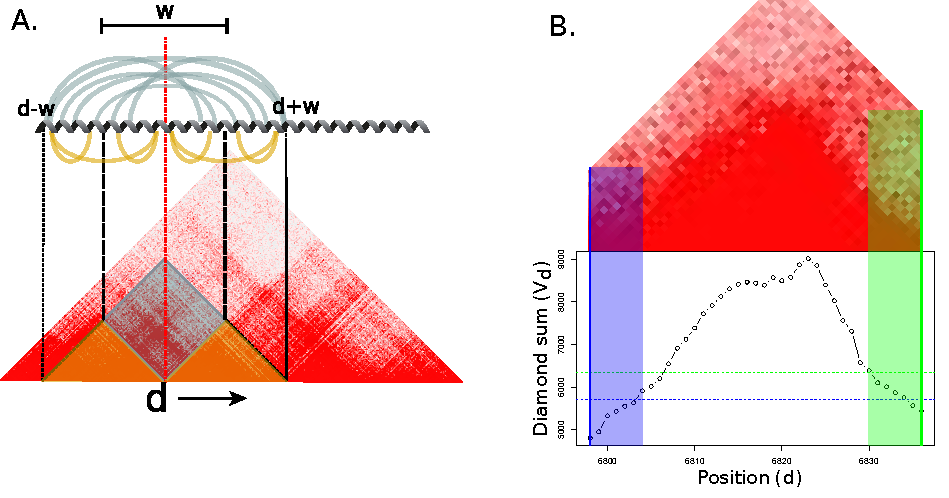
\includegraphics[width=1\textwidth]{Figures/6_interactions.pdf}
	\caption{Visual representation of the algorithm used to compute TAD boundaries in Hi-C matrices. \textbf{A.} A diamond (blue) of width $w$ set to 100kb is slid on all positions ($d$) along the diagonal of each intrachromosomal contact matrix. \textbf{B.} At each position $d$, the sum of all values in the diamond ($V_d$) is computed. The sum is not computed at the first and last $w$ positions as the diamond would be outside the matrix limits. \textbf{C.} For each TAD, boundary regions are extended inwards from its borders until the sum recorded by the diamond ($V_d$) has increased its original value at the border by 10\% of the maximum value in the TAD. The solid vertical lines represent the TAD borders, the horizontal dashed lines represent the thresholds required to stop extending boundaries and the transparent areas represent the final boundaries. All blue elements relate to the left side of the TAD, while all green elements relate to the right side.}
	\label{interact_hic}
\end{figure}

\FloatBarrier
\section*{Discussion}

Although it has been long recognized that chromosomal conformation has strong impact on the regulation of gene transcription programs, features that underlie the regulation of chromatin organization remain relatively unclear \cite{Bonev2016}⁠. Following the development of chromosome conformation capture techniques over a decade ago \cite{Dekker2002}⁠, advances in other 3C-based technologies have allowed the quantification of chromosomal interaction frequencies between genomic loci in close spatial proximity, both locally (i.e. 3C and 4C) and genome-wide (i.e. Hi-C and ChIA-PET) \cite{Dekker2013}.

LincRNAs originating from enhancers (elincRNAs) have been proposed to modulate chromosomal architecture \cite{Yin2015}⁠ and are frequently located within topologically associating domains (TADs) where high levels of genomic interactions occur compared to other expressed lincRNAs (Tan et al, 2016, under revision). Here, I used publicly available genomics data to investigate the prevalence of elincRNA regulation in modulating chromosomal architecture. Together with strong enrichment in cohesin binding at elincRNAs promoter regions, their frequent localization at loop anchors and association with high amount of intra-TAD contacts support their putative role in regulating enhancer-promoter loops. 

There is ongoing debate on the biological relevance of elincRNA transcription in particular with regards to  whether their associated regulatory roles are transcript- or transcription-dependent. Notably, although the association between elincRNA expression and high frequency of chromosomal interactions suggests their putative function, this might be driven by the enhancer activities, rather than the elincRNA itself. Comparing elincRNAs to active enhancers that only produce unstable and bidirectionally-transcribed eRNAs can provide initial insights to  this key question. Ultimately, the dissection of the molecular mechanisms underlying enhancer-mediated regulation of chromosomal conformation will require genetic manipulations of elincRNA transcript abundances (i.e. by RNAi) and inhibiting their transcription (i.e. with CRISPRi) \cite{Li2013}⁠.

Furthermore, extending this analysis, which focuses on within-topological domain interactions to between-TAD contacts (i.e. meta-TADs) \cite{Fraser2015}⁠, to inter-chromosomal contacts, and eventually to DNA associations with the nuclear lamina would provide a more complete and global overview of elincRNA-dependent chromosomal interactions. These analyses could also be extended to additional cell-lines to investigate whether the effect of elincRNAs in nuclear architecture is cell-line specific, or more generalized. 

The current resolution of global chromosomal conformation capture techniques (including Hi-C) remains a limiting factor to measure accurate interaction frequencies at elincRNA loci as it is presently not possible to confidently examine contacts in regions smaller than the Hi-C resolution \cite{Rao2014}⁠. Instead, only an estimation of the region surrounding the gene can be measured. In addition, even using data with relatively high contact resolutions, bulk Hi-C technique provides only a mean estimate of all chromosomal contacts within a cell population, thus averaging out the cell-to-cell dynamics and variabilities. Recently, a single-cell Hi-C technique has been developed \cite{Nagano2013}⁠, allowing one to examine DNA contact profiles at a single cell resolution, although the precision of the method likely requires improvement. Such single cell techniques, combined with higher contact resolution, would provide greater power to investigate the impact of elincRNAs on chromosome architecture.

\section*{Materials and methods}
Unless stated otherwise, all statistical tests were performed using R 3.3.1 \cite{RCoreTeam2016}⁠. Overlapping of genomic elements were done using either bedtools 2.26 \cite{Quinlan2010} ⁠or the “intervals” package \cite{Bourgon2015}⁠ in R. Manipulations of Hi-C contact matrices were performed using the “Matrix” R package \cite{Bates2016}⁠. All positions of genetic elements used are based on the hg19 human assembly.

\subsection*{elincRNA definition}

LCL-expressed lincRNAs and protein-coding genes sets were provided by Jennifer Tan. Briefly, they include all lincRNAs and protein-coding genes annotated in GENCODE (version19) and \textit{de novo} LCL-expressed lincRNAs assembled using RNA sequencing reads from ENCODE GM12878 cell-line (Tan et al, 2016, under revision). elincRNAs were classified as lincRNAs whose putative promoter regions (Figure \ref{Genome_browser}), defined as the 1kb region upstream from the transcription start site overlap predicted enhancers in GM12878 using histone marks \cite{ENCODEProject2012}⁠. LincRNAs whose promoter region overlap predicted active promoter regions were excluded from the analysis.

\subsection*{Expression levels}

Expression levels for elincRNAs and protein-coding genes in 4  different cell lines (GM12878, HUVEC, K562 and NHEK) were estimated by Jennifer Tan using RNA sequencing data generated by the ENCODE consortium \cite{ENCODEProject2012}. Specifically, reads that overlap exons of lincRNAs and protein-coding genes (GENCODE version 19) were used to estimate their expression levels (in RPKM) in each sample.

\subsection*{Conservation and tissue specificity}

Sequence conservation of gene exons across mammalian and primate evolution were estimated using phastCons scores \cite{Siepel2005}⁠, a measure of exonic sequence conservation, by Jennifer Tan. Tissue specificity index (Tau) was computed following the procedure described in \cite{Kryuchkova2015a}, considering only genes with expression above a cutoff of 0.1 RPKM.

\subsection*{Chip-seq data}

Peaks for CTCF, RAD21 and SMC3 in GM12878 were obtained from the ENCODE consortium ChIP sequencing data \cite{ENCODEProject2012}⁠. Cohesin peaks were defined as the union between the peaks of RAD21 and SMC3. The non-overlapping CTCF and cohesin peaks were obtained by excluding peaks common to both CTCF and cohesin binding.

\subsection*{Enrichment of genetic elements}

All enrichment tests were performed using the genome association tester (GAT)⁠ version 1.2. This tool tests for enrichment in the number of observed overlap between lincRNAs and genomic elements compared to what would be expected if they were distributed randomly. The null distribution was obtained by randomly sampling 10,000 times (with replacement) segments of the same length and matching GC content as the tested loci across the intergenic regions of the human genome. Enrichment of loop anchors at TAD boundaries was compared to random regions of the same size randomly placed across the whole genome. To control for potential confounding variables that correlate with GC content, such as gene density, the genome was divided into segments of 10 Kb and assigned to eight isochore bins in the enrichment analysis. The GC content of each bin was as follows: 0-36, 36-38, 38-40, 40-42, 42-44, 44-46, 46-48, 48-100 \cite{Heger2013}. 

For all enrichment tests, two values are reported in the results section: Fold enrichment and q-value. Fold enrichment corresponds to the ratio between observed and median expected number of segment overlaps. Fold enrichments above 1 indicate the tested segments are enriched compared to random expectation, whereas those below 1 represent depletion in observed overlaps. The q-values are adjusted p-values using the Benjamin-Hochberg multiple-testing correction.

\subsection*{Hi-C data and normalization}

All chromosomal interactions were estimated using 5kb resolution Hi-C intrachromosomal contact matrices constructed from all mapped read pairs with MAPQ scores of at least 30 \cite{Rao2014}. To correct for bias induced by chromatin accessibility and restriction sites frequency across the genome \cite{Rao2014}, matrices were normalized using the provided KR normalization vector for all cell lines, except for chromosome 9, where the SQRTVC (square root vanilla coverage) was used as the KR algorithm did not reach convergence for this chromosome in K562, likely due to the high sparsity of the matrix. I chose SQRTVC as this method yields very similar results to KR. 
The normalization procedure, as described by the authors, sequentially divides each entry in the raw contact matrix $M$ by its corresponding values in the normalization vector $N$:

\vspace{0.2in}
$M^*_{i,j}=\frac{M_{i,j}}{N_{[\frac{i}{res}]}*N_{[\frac{j}{res}]}}$
\vspace{0.2in}

\noindent Where $M_{i,j}$ is an entry from the raw matrix and $M^*_{i,j}$ corresponding normalized entry and $res$ is the resolution of the contact matrix (i.e. 5000, in this study).

\subsection*{TAD definition}

List of TADs coordinates in 4 different cell lines (GM12878, HUVEC, K562 and NHEK) used in the computations were obtained from \cite{Rao2014}. They called TADs based on Hi-C data across several human cell lines, normalized and processed with their own algorithm. Here, all the large TADs that completely encompass smaller ones were removed from the analysis to focus on low-level interactions within TADs and not interactions occurring between TADs (i.e. building higher level meta-TADs \cite{Fraser2015}).

\subsection*{TAD boundaries definition}

TAD boundaries were defined using a custom algorithm based on the assumption that there are few interactions between elements located before and those after the boundaries. These interactions are measured by sliding the corner of a diamond of width $w$ (Figure \ref{interact_hic}A) on every position $d$ along diagonal of a square matrix $M$ of $n$ dimensions. The sum of interactions in the diamond is computed at each position $d$ between $1+w$ and $n-w$ (Figure \ref{interact_hic}B). The limits of $d$ were set to prevent the diamond from exceeding the limits of the matrix. The computed sum of interactions at each position $d$ is stored in a vector $V$. This can be rewritten as: 

\vspace{0.2in}
$\left\{\begin{matrix}1\leq w\leq \frac{n}{2} \\ \forall d\in\left \{ 1+w , ... , n-w \right \}\end{matrix}\right. V_{d}=\sum_{i=d-w}^{d}\sum_{j=d}^{d+w}M_{i,j}$
\vspace{0.2in}

\noindent The size of the diamond ($w$) was set to 100kb, based on the fact that the median length of filtered TADs is 140kb.

For each TAD, boundary regions are extended inwards from the borders (Figure \ref{interact_hic}C) as long as the value of $V$ does not exceed an arbitrary threshold defined as the starting value (at the TAD border) plus 10\% of the maximum value in the TAD (Figure \ref{interact_hic}B).I discarded TAD boundaries which encompassed their whole TAD. These boundaries failed to stop due to TADs presenting relatively low differences between the contacts at their borders and their maximum value.

\subsection*{intra-TAD contacts}

The mean frequency of contact was estimated for each TAD that overlap a gene of interest (Figure \ref{interact_hic}B). For genes that overlap multiple TADs, contacts within each of the overlapping TAD is computed independently.

\section*{Acknowledgements}
I wish to thank Jennifer Yihong Tan for her precious advices and help throughout the project and writing of the report. I also wish to thank Ana Claudia Marques for her suggestions, general guidance and corrections in the report. Finally, I want to thank Adam Alexander Thil Smith for his help with technical issues and code optimization and Maria Ferreira da Silva for her suggestions and critical reading of the report.
Computationally demanding analyses were performed at the Vital-IT Center for High Performance Computing of the Swiss Institute of Bioinformatics (www.vital-it.ch).

\section*{Supplementary Material}
Code and manuscript data hosted at: \url{https://github.com/cmdoret/FSP_MLS}

\noindent Raw contact matrices and normalization vector available at: \url{https://www.ncbi.nlm.nih.gov/geo/query/acc.cgi?acc=GSE63525}

\noindent \textit{In situ} primary + replicates intrachromosomal contact matrices were used for GM12878. Intrachromosomal matrices were used fo all other cell lines.

%\bibliography{First_step}{}
\bibliographystyle{apalike}
\fancyhead[L]{\slshape }
\bibliography{firststep}
\end{document}